% !TEX program = tectonic
\documentclass[UTF8,11pt,a4paper]{ctexart}

\usepackage[a4paper,margin=2.2cm,headheight=15pt]{geometry}
\usepackage{amsmath,amssymb,bm}
\usepackage{booktabs,longtable,tabularx,array,multirow}
\usepackage{graphicx,float,subcaption}
\usepackage{xcolor}
\usepackage{tikz}
\usetikzlibrary{arrows.meta,positioning,fit,shapes.geometric}
\usepackage{hyperref}
\usepackage{fancyhdr}
\usepackage{enumitem}
\usepackage{listings}
\usepackage{siunitx}
\usepackage{microtype}

\definecolor{igemgreen}{HTML}{176B57}
\definecolor{igemblue}{HTML}{2C6E9B}
\definecolor{igemorange}{HTML}{D17A22}
\definecolor{lightgreen}{HTML}{EAF4EF}
\definecolor{lightblue}{HTML}{EDF4F8}
\definecolor{lightgray}{HTML}{F4F5F6}
\definecolor{warning}{HTML}{8A5A12}

\hypersetup{
  colorlinks=true,
  linkcolor=igemgreen,
  citecolor=igemblue,
  urlcolor=igemblue,
  pdftitle={AAV-SINEUP 多尺度递送建模模拟},
  pdfauthor={PekingHSC iGEM Dry Lab 朱子轩}
}

\pagestyle{fancy}
\fancyhf{}
\fancyhead[L]{AAV--SINEUP Spatial PK}
\fancyhead[R]{PekingHSC iGEM Dry Lab 朱子轩}
\fancyfoot[C]{\thepage}

\setlength{\parindent}{2em}
\setlength{\parskip}{0.35em}
\setlength{\emergencystretch}{1.5em}
\setlist[itemize]{leftmargin=2em,itemsep=0.25em,topsep=0.35em}
\setlist[enumerate]{leftmargin=2.2em,itemsep=0.25em,topsep=0.35em}
\renewcommand{\arraystretch}{1.25}
\graphicspath{{../../results/mouse_pbpk/}}

\newcommand{\vg}{\mathrm{vg}}
\newcommand{\AUC}{\mathrm{AUC}}
\newcommand{\dd}{\mathrm{d}}
\newcommand{\code}[1]{\texttt{#1}}
\newcommand{\status}[1]{\textcolor{igemgreen}{\textbf{#1}}}
\newcommand{\assumption}[1]{\textcolor{warning}{\textbf{建模假设：}#1}}

\lstset{
  basicstyle=\ttfamily\small,
  backgroundcolor=\color{lightgray},
  frame=single,
  rulecolor=\color{gray!30},
  breaklines=true,
  columns=fullflexible,
  keepspaces=true,
  showstringspaces=false
}

\title{\vspace{-1.2cm}\textbf{AAV--SINEUP 多尺度递送与 Spatial PK 项目报告}\\[0.6em]}
\author{PekingHSC iGEM Dry Lab 朱子轩}
\date{2026 年 8 月}

\begin{document}
\maketitle

\begin{center}
\begin{minipage}{0.92\textwidth}
\end{minipage}
\end{center}

\begin{abstract}
针对染色体缺失与单倍剂量不足疾病，本项目探索用 AAV 递送一个或多个 SINEUP 元件，增强患者剩余正常等位基因 mRNA 的翻译。第一阶段在小鼠尺度建立 64 状态机制模型，包含 8 个器官 PBPK、肝细胞转导、肾近端小管双入口、BBB/CNS 转导、免疫与质量守恒。第二阶段保留相同的 $Q$--$PS$--$K_p$--受体--episome 方程族，将系统扩展为 70 kg 参考成人、24 个解剖区域、301 个状态、显式心肺/门静脉循环以及 IV、IT、IM、ICM、ICV 和吸入六种给药途径。批量导出器对 8 种衣壳逐一重求解； 项目中使用 GTEx 与 Human Protein Atlas 提供 42 个疾病基因的健康组织表达先验；React 前端将 ODE 结果展示为器官特异性--单次给药持久性二维图、人体时空热图和带给药/免疫负担惩罚的探索性组合方案。
\end{abstract}

\tableofcontents
\clearpage

\section{生物学问题与工程目标}

\subsection{为什么选择 AAV--SINEUP 组合}
许多单倍剂量不足疾病并不是完全缺失目标蛋白，而是一个等位基因失活或一段染色体缺失后，正常等位基因的表达量不足。SINEUP 是一类具有反义结合域和翻译增强效应域的非编码 RNA，可在不改变靶 mRNA 序列的前提下提高其翻译效率\cite{sineup2015}。因此，本项目的治疗构想是：
\begin{enumerate}
  \item 根据疾病、缺失区段和残余正常等位基因选择 SINEUP 靶标；
  \item 选择能够到达目标器官和目标细胞层次的 AAV 衣壳；
  \item 通过组织/细胞特异性调控控制脱靶表达；
  \item 用模型预测递送量、转导瓶颈和单次给药的有效窗口；
  \item 将预测送回湿实验，以更少的组合完成验证。
\end{enumerate}

该方案的关键困难在于，AAV 的“体内出现”并不等于“目标蛋白恢复”。从静脉给药到作用形成至少经历血液清除、器官分布、屏障跨越、受体结合、内吞、内体逃逸、入核、解包、双链化、episome 形成、RNA 表达和蛋白周转。模型的核心价值正是把这些步骤拆开，使每个设计变量对应可解释的生物学环节。

\subsection{本项目尝试解决的问题}
\begin{itemize}
  \item 普通 AAV9 静脉给药后，肝、脾、肾、心、肌肉、肺、脑和其余组织的早期暴露如何比较？
  \item 肝脏、肾近端小管和 CNS 的细胞内转导链分别有哪些瓶颈？
  \item BBB 跨越和 CNS 深度分布如何影响神经系统疾病的衣壳排序？
  \item 如何把 ODE 输出转化为用户可交互的二维设计空间？
  \item 如何进一步耦合流体力学，得到真正的 spatial PK？
\end{itemize}

\section{Engineering：Design--Build--Test--Learn}

本项目把模型视为可被测量和修正的工程对象，而不是一次完成的插图。每次迭代均采用四项验收标准：给药量与所有载体状态及累计 sink 闭合；求解成功且无有意义的负状态；capsid、vector genome、episome、RNA 和蛋白不被混作同一读数；相同命令可以重新生成前端数据。通过这些检查只说明计算内部一致，不等于参数或临床结论正确。

\small
\begin{longtable}{p{0.09\textwidth}p{0.17\textwidth}p{0.21\textwidth}p{0.18\textwidth}p{0.22\textwidth}}
\toprule
迭代 & Design & Build & Test & Learn \\
\midrule
\endfirsthead
\toprule
迭代 & Design & Build & Test & Learn \\
\midrule
\endhead
1：衰减 & 替代仅为画出钟形曲线的统一半衰期 & 显式血液、血管/RES、ISF 损失及累计 sink；拟合 AAV9 器官表观半衰期 & 质量守恒达到数值精度；保留拟合诊断 & 现有数据不能识别血管与 ISF 两个速率，35:65 拆分必须标为结构假设 \\
2：转导 & 解释相似器官暴露为何产生不同表达 & 肝、肾双入口和 BBB/CNS 胞内链 & 分别改变 capsid transport、escape 与 promoter & 增加 episome 不一定同比增加蛋白；湿实验必须分层测量 \\
3：人体投影 & 避免把小鼠按体重直接放大 & 心肺/门静脉、24 区域、301 状态、六种给药入口 & 血容量、流量闭合、CSF 周转和逐途径质量守恒 & 人体解剖可以有依据，但衣壳转化仍是不确定先验 \\
4：设计工具 & 让用户从疾病/基因而非状态名进入 & 批量求解、JSON/CSV、二维图与人体热图 & 前端构建测试、绝对/相对色标、固定 UTC 元数据 & 相对色标利于看格局但会隐藏绝对下降，必须保留两种尺度 \\
\bottomrule
\end{longtable}
\normalsize

本轮代码审计还发现肝转录 Hill 输出曾被硬编码为不超过 2.0，导致高于 2.0 的 promoter preset 不能完整生效；现已改为不超过该场景自己的 \code{k\_tx}。这类失败被保留在工程记录中，因为它解释了为什么过去某些参数变化没有产生预期输出。


\section{总体模型架构}

\begin{figure}[H]
\centering
\resizebox{\textwidth}{!}{%
\begin{tikzpicture}[
  node distance=7mm and 9mm,
  box/.style={draw,rounded corners=2pt,align=center,minimum height=10mm,minimum width=28mm,fill=lightblue},
  organ/.style={draw,rounded corners=2pt,align=center,minimum height=10mm,minimum width=28mm,fill=lightgreen},
  arrow/.style={-{Latex[length=2.2mm]},thick,draw=gray!75}
]
\node[box] (dose) {疾病/基因\\衣壳/途径};
\node[box,right=of dose] (blood) {给药入口\\blood/CSF/depot};
\node[organ,right=of blood] (pbpk) {鼠 8 器官 / 人 24 区域\\vascular $\leftrightarrow$ ISF};
\node[organ,below left=of pbpk] (liver) {肝细胞\\binding $\to$ episome};
\node[organ,below=of pbpk] (kidney) {肾近端小管\\双入口转导};
\node[organ,below right=of pbpk] (cns) {BBB + CNS\\细胞转导};
\node[box,below=18mm of kidney] (expr) {mRNA / SINEUP RNA\\蛋白恢复};
\node[box,right=of expr] (space) {CNS 深度模型\\1D/未来 3D spatial PK};
\node[box,left=of expr] (audit) {累计 sinks\\质量守恒审计};
\node[box,below=of expr] (ui) {GTEx/HPA + ODE 输出\\二维图/人体热图/组合筛选};
\draw[arrow] (dose) -- (blood);
\draw[arrow] (blood) -- (pbpk);
\draw[arrow] (pbpk) -- (liver);
\draw[arrow] (pbpk) -- (kidney);
\draw[arrow] (pbpk) -- (cns);
\draw[arrow] (liver) -- (expr);
\draw[arrow] (kidney) -- (expr);
\draw[arrow] (cns) -- (expr);
\draw[arrow] (cns) -- (space);
\draw[arrow] (expr) -- (audit);
\draw[arrow] (expr) -- (ui);
\draw[arrow] (space) -- (ui);
\end{tikzpicture}
}
\caption{当前多尺度计算框架。疾病定义靶点，衣壳和途径定义输入；PBPK 提供器官边界暴露，细胞转导产生 episome，SINEUP-PD 产生蛋白恢复。}
\label{fig:architecture}
\end{figure}

模型采用“量（amount）作为状态、浓度用于通量计算”的方式。这样不同有效体积之间的交换可以统一写成质量通量，且所有 AAV 状态与损失 sink 能够直接相加进行质量守恒审计。当前并行维护两条支路：\code{ode1.0.py} 是 64 状态鼠机制模型，保留最细的肝、近端小管和 BBB 细胞过程；\code{human\_spatial\_pbpk.py} 是 301 状态参考成人模型，强化循环拓扑、区域空间和给药入口。二者共享局部器官方程，但用途与证据层级不同。

\section{全身 PBPK 模型}

\subsection{给药输入}
默认总剂量为 $D=10^{12}\,\vg$，在 $T_{inf}=10$ min 内以零级速率输入：
\begin{equation}
R_{in}(t)=
\begin{cases}
D/T_{inf}, & 0\le t\le T_{inf},\\
0, & t>T_{inf}.
\end{cases}
\end{equation}
代码同时支持 bolus 初始条件，便于比较给药方式对早期峰值的影响。

\subsection{血液--器官血管--间质交换}
对器官 $i$，定义
\begin{equation}
C_b=\frac{A_b}{V_b},\qquad C_{v,i}=\frac{A_{v,i}}{V_{v,i}},\qquad C_{isf,i}=\frac{A_{isf,i}}{V_{isf,i}}.
\end{equation}
血液到器官血管的有效交换通量与血管到间质的通量分别为
\begin{align}
J_{b\to v,i} &= Q_i(C_b-C_{v,i}),\\
J_{v\to isf,i} &= PS_i\left(C_{v,i}-\frac{C_{isf,i}}{K_{p,i}}\right).
\end{align}
其中 $Q_i$ 是有效灌流/交换参数，$PS_i$ 是通透性--表面积乘积，$K_{p,i}$ 是组织分配系数。基本状态方程为
\begin{align}
\frac{\dd A_b}{\dd t} &= R_{in}-\sum_iJ_{b\to v,i}-J_{blood\,clear}-J_{neut},\\
\frac{\dd A_{v,i}}{\dd t} &= J_{b\to v,i}-J_{v\to isf,i}-J_{res,i}+J_{return,i},\\
\frac{\dd A_{isf,i}}{\dd t} &= J_{v\to isf,i}-J_{deg,isf,i}-J_{cell,i}+J_{recycle,i}.
\end{align}
脑、肾和肝的细胞摄取会进一步修改对应的 $J_{cell,i}$；BBB 回收、肾内体回收等则通过 $J_{return}$ 或 $J_{recycle}$ 返回外部池。

\subsection{衰减方程}
一阶半衰期衰减的数学形式为
\begin{equation}
\frac{\dd A}{\dd t}=-kA,\qquad k=\frac{\ln2}{t_{1/2}},\qquad A(t)=A_0e^{-kt}.
\end{equation}
目前方程的其中一个问题是未说明 AAV 去了哪里。
代码中我加入了 \code{mechanistic} 模式把损失写入明确的累计通道：中央血液清除、器官血管/内皮清除、间质降解、抗体中和、肝细胞内损失、肾尿排与胞内降解、BBB/CNS 降解。并通过质量守恒的方式验证。器官半衰期先验仍通过 $k=\ln2/t_{1/2}$ 转成速率，但当前暂按
\begin{equation}
k_{res,i}=0.35\frac{\ln2}{t_{1/2,i}},\qquad
k_{deg,isf,i}=0.65\frac{\ln2}{t_{1/2,i}}
\end{equation}
分配到血管/内皮与 ISF 两个去向。

\begin{table}[H]
\centering
\caption{当前普通 AAV9 早期完整/标记 capsid 半衰期先验。单位为小时。}
\begin{tabular}{lrrrrrrrrr}
\toprule
器官 & 血液 & 肝 & 脾 & 肾 & 心 & 肌肉 & 肺 & 脑 & 其余 \\
\midrule
$t_{1/2}$ & 2.4 & 22.6 & 22.9 & 24.0 & 15.6 & 48.7 & 18.0 & 24.8 & 34.0 \\
\bottomrule
\end{tabular}
\end{table}
血液、肝、心、脾、脑/CSF 和全身值主要参考放射标记 AAV 的早期成像研究所得\cite{ballon2020}；肾与肺当前是明确标注的 provisional mouse-scale prior。放射信号、完整有感染能力的 capsid、vector genome 和表达性 episome 是不同 analyte，不能混为同一个半衰期\cite{bioanalytical2023}。

\begin{figure}[H]
\centering
\begin{subfigure}{0.49\textwidth}
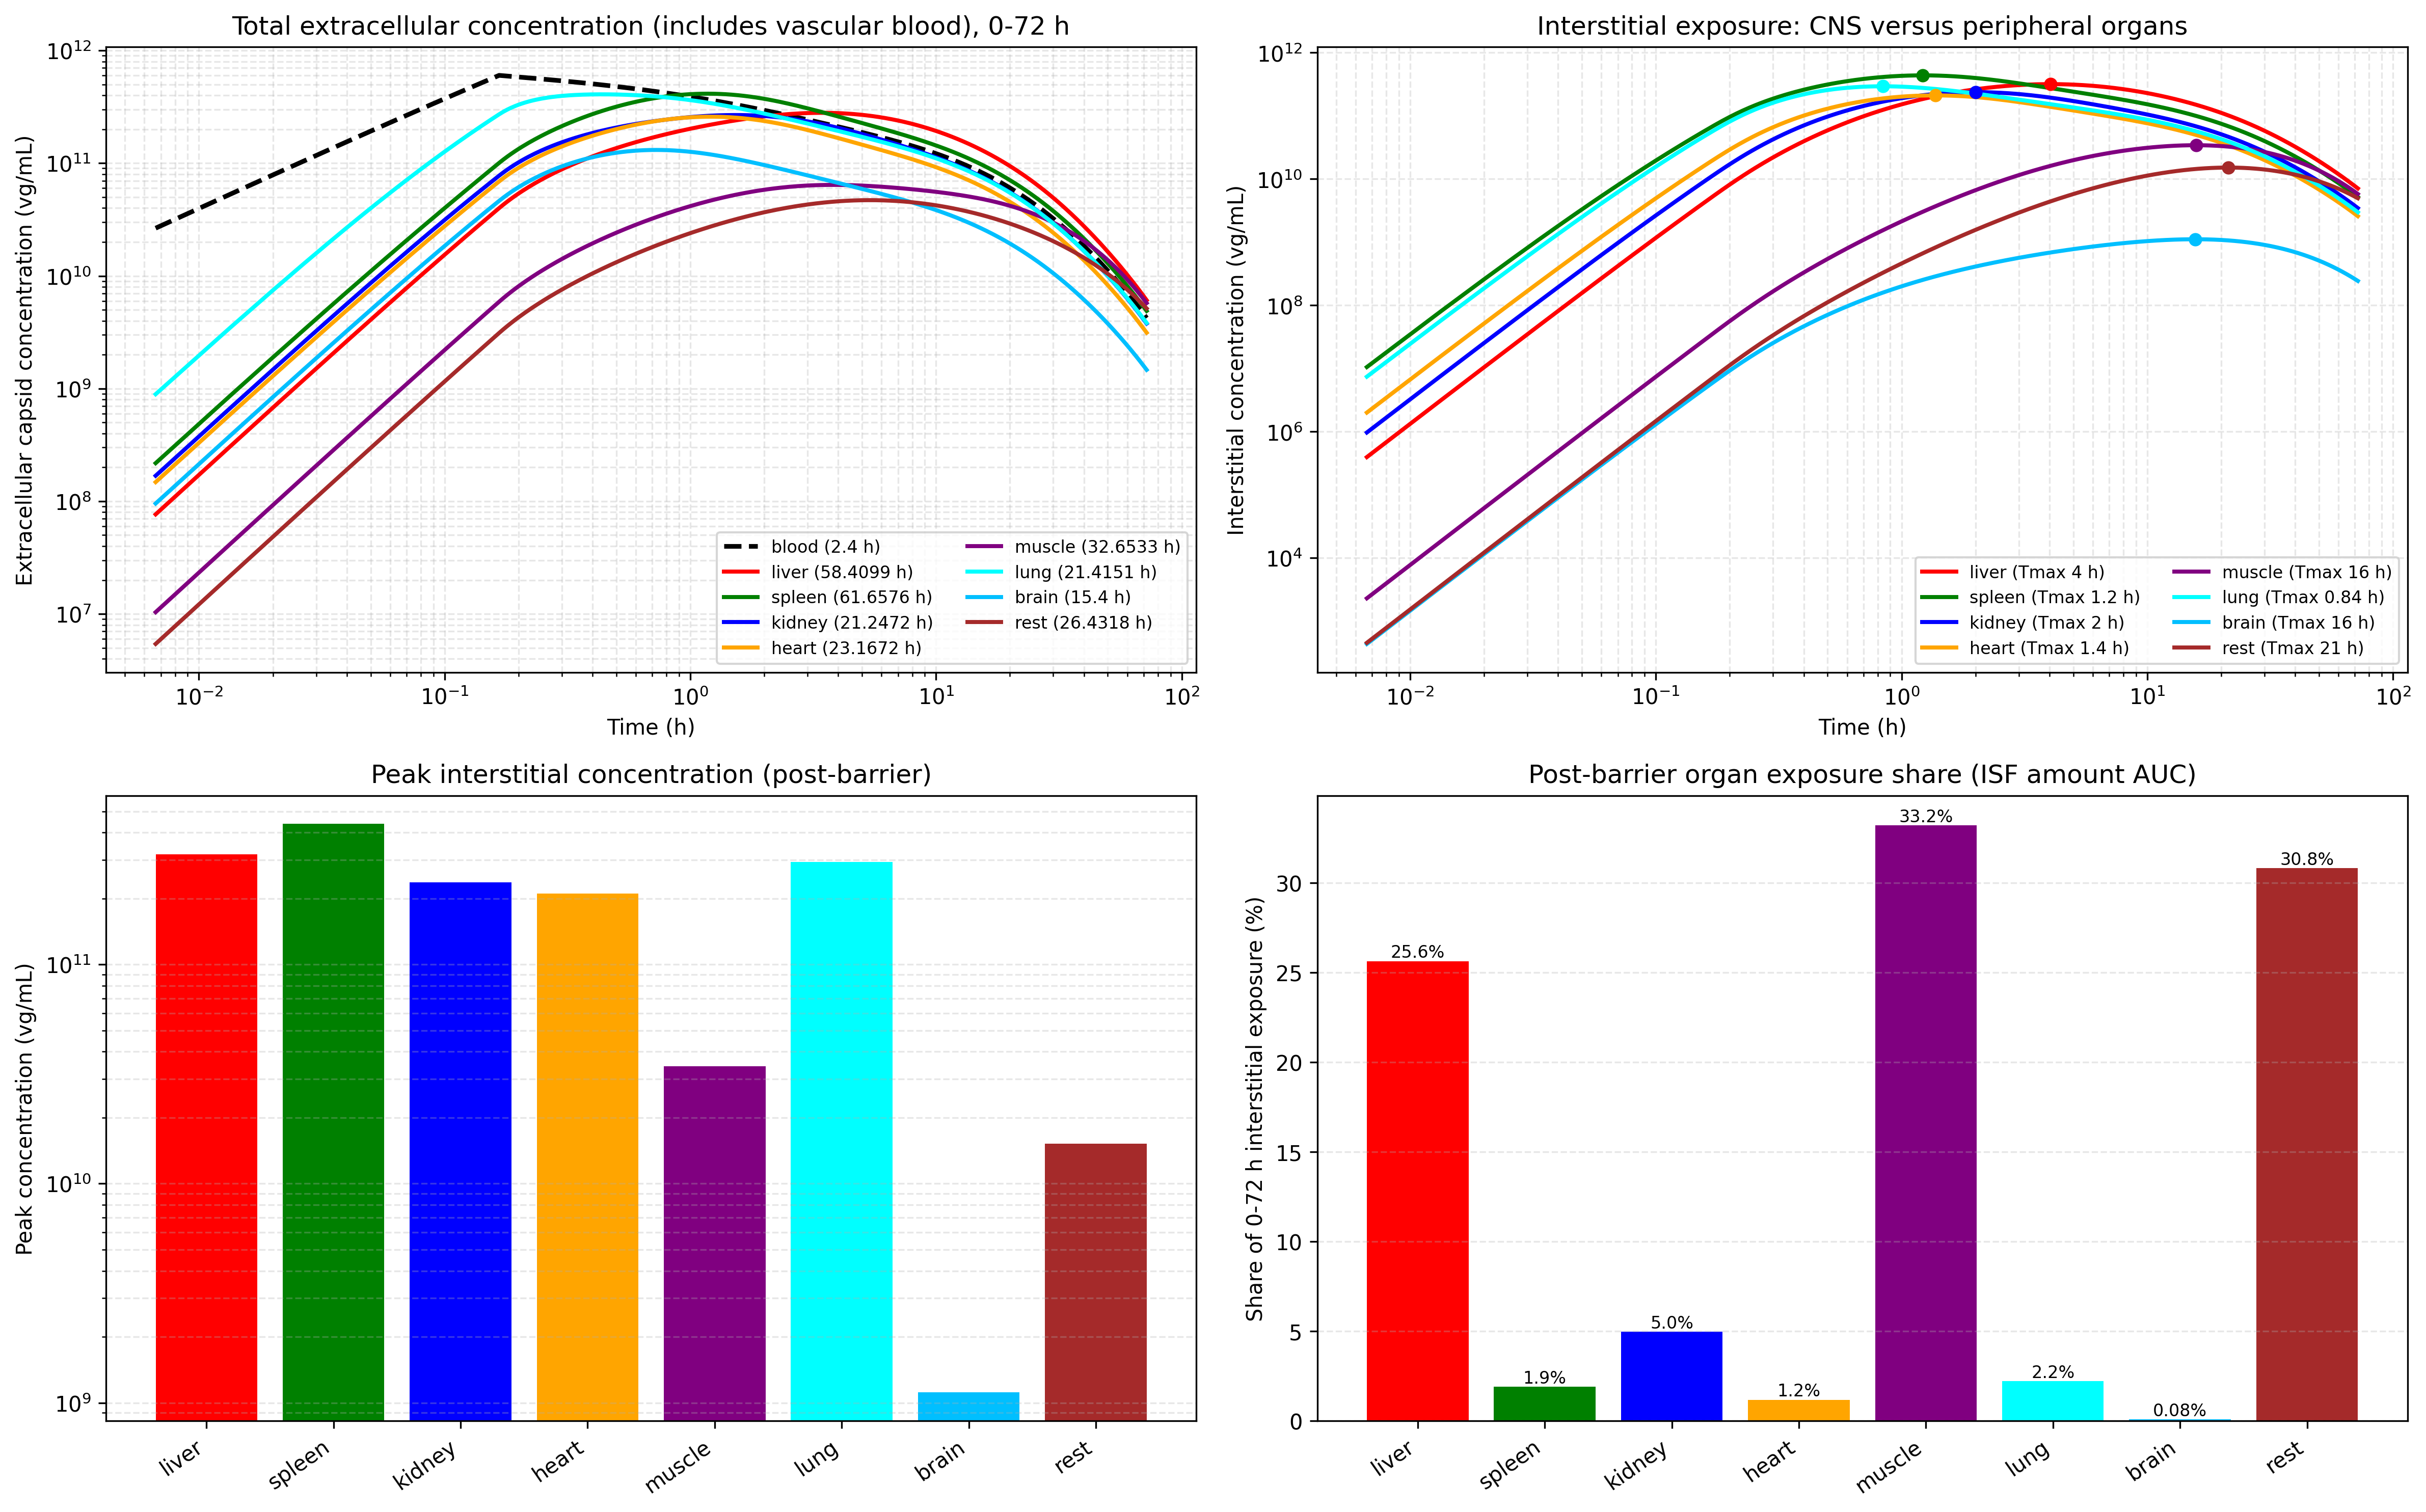
\includegraphics[width=\linewidth]{13_normal_aav9_organ_concentration_comparison_log_axes.png}
\caption{双对数轴，显示分钟至天的峰值与衰减。}
\end{subfigure}
\begin{subfigure}{0.49\textwidth}
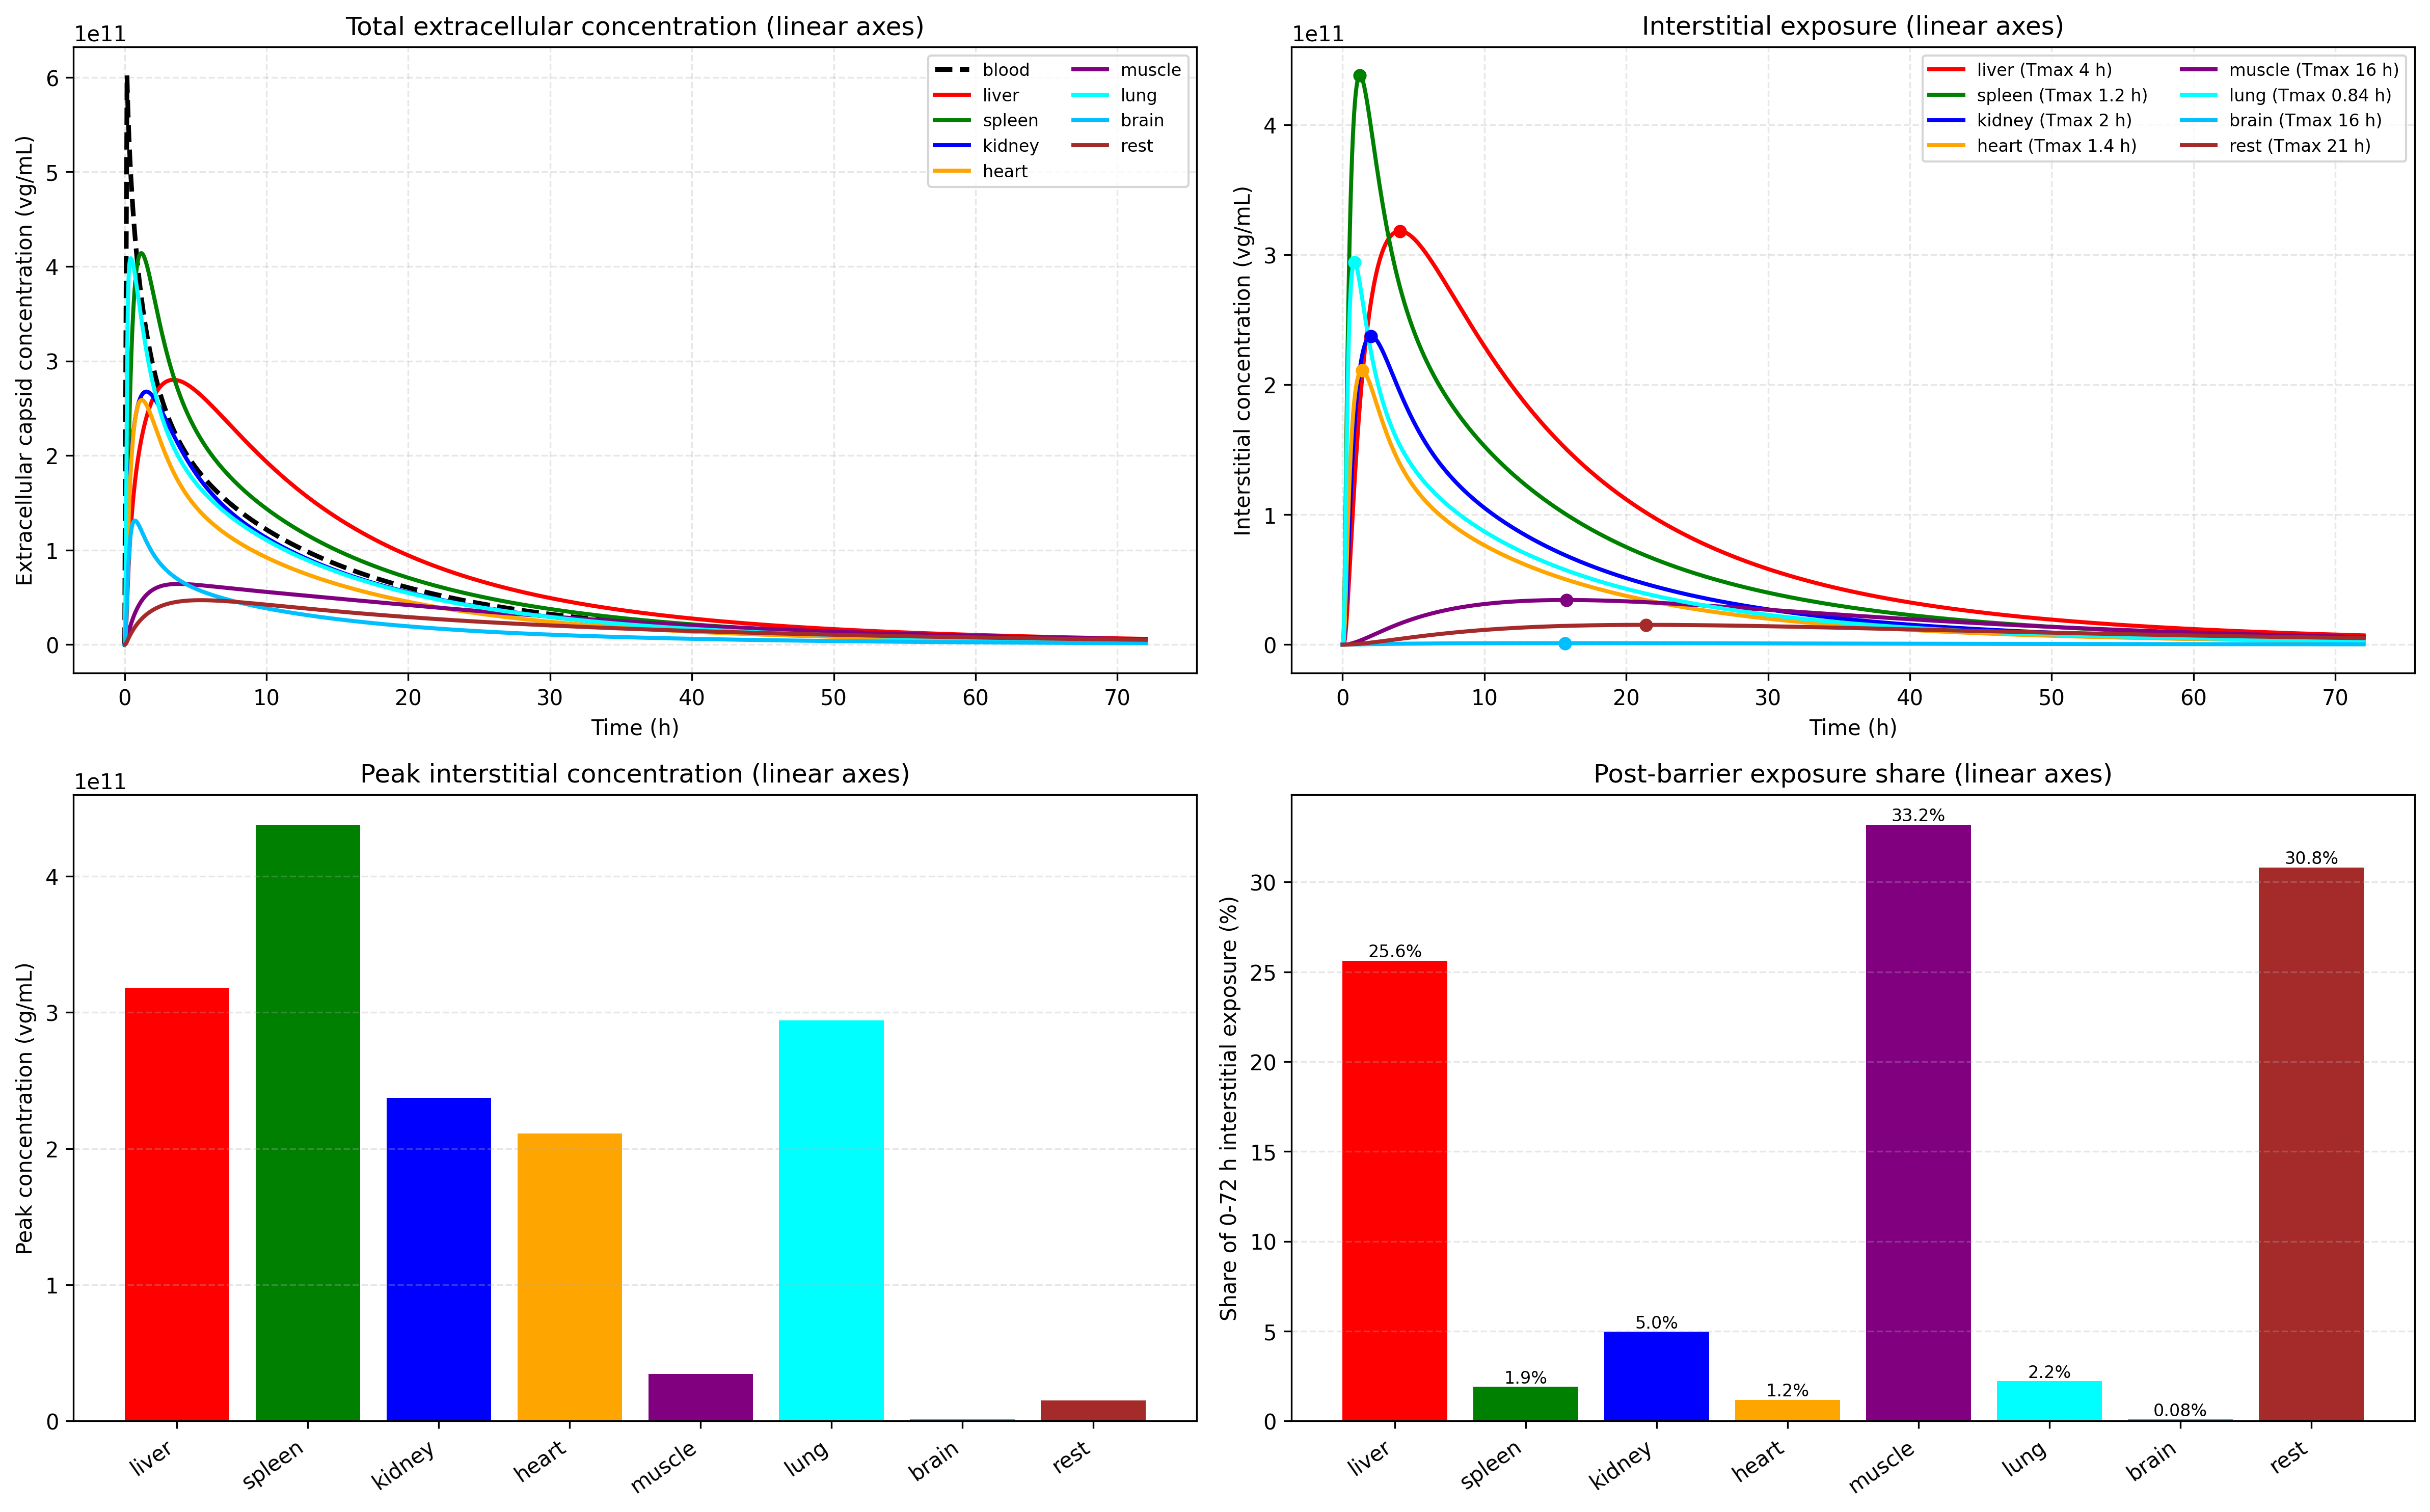
\includegraphics[width=\linewidth]{14_normal_aav9_organ_concentration_comparison_linear_axes.png}
\caption{线性轴，显示绝对时间尺度。}
\end{subfigure}
\caption{普通 AAV9-like 基线的多器官浓度比较。}
\label{fig:organ}
\end{figure}

\section{70 kg 参考成人多区域模型}

\subsection{为什么不能按体重直接放大小鼠模型}
小鼠模型的剂量、血容量、心输出量和器官体积不能用同一个体重倍数外推。人体模型因此保留局部器官方程，但重新定义循环拓扑、区域体积、血流份额、$PS$、$K_p$、受体容量和持久性。参考个体体重为 70 kg，剂量为 $4\times10^{13}$ vg/kg，即总量 $2.8\times10^{15}$ vg。成人心输出量先验为 $330$ L/h；为保持与原集中室模型一致的有效交换时间尺度，求解中仍使用
\begin{equation}
Q_{effective}=0.05\,Q_{physiological}.
\end{equation}
这一缩放是建模折中，不表示真实人体心输出量只有生理值的 5\%。前端同时保存生理血流与实际进入交换方程的有效血流，避免二者混淆。

\begin{table}[H]
\centering
\caption{鼠机制模型与参考成人模型的结构对照。}
\begin{tabularx}{\textwidth}{p{0.22\textwidth}XX}
\toprule
项目 & 64 状态鼠模型 & 301 状态参考成人模型 \\
\midrule
循环 & 单一中央血池并联 8 个器官 & 手臂静脉、右心、肺动脉/静脉、左心、动脉、静脉 \\
空间 & 每器官 vascular + ISF & 24 个区域，每区 vascular、ISF、受体、胞内链、episome、mRNA、蛋白 \\
肝回流 & 直接连中央血池 & 肝动脉加肠道/脾脏门静脉输入 \\
CNS & 单一脑血管/ISF + BBB；另接三级深度降阶模型 & 7 个脑/脊髓区 + 腰段/颅内 CSF + 途径特异区域入口 \\
肾脏 & 单肾室但含滤液、管腔、顶端/基底外侧摄取 & 左右肾皮质/髓质；当前使用统一胞内链，尚未嵌入完整管腔模型 \\
主要用途 & 机制解释与二维设计点 & 人体首过、区域达峰、给药途径比较和热图 \\
\bottomrule
\end{tabularx}
\end{table}

\subsection{显式心肺与门静脉循环}
外周静脉给药首先进入注射侧手臂静脉，随后依次经过右心、肺动脉、肺、肺静脉、左心与体循环动脉。以右心和体循环器官为例：
\begin{align}
\dot A_{RH}&=J_{arm\to RH}+Q_{eff}(C_{ven}-C_{RH})-J_{clear,RH},\\
\dot A_{v,i}&=Q_i(C_{art}-C_{v,i})-PS_i\left(C_{v,i}-\frac{C_{isf,i}}{K_{p,i}}\right)-J_{loss,v,i}.
\end{align}
肺区从肺动脉接收输入并汇入肺静脉；肝脏则接收肝动脉、肠道门静脉和脾静脉三部分输入。该拓扑能够产生注射点、肺首过、肝门静脉回流及不同区域 $Q/V$ 所导致的达峰差异，而原中央血池模型不能解析这些先后关系。

\subsection{24 个区域与 301 个状态}
人体模型包含额叶、顶叶、颞叶、枕叶、深部灰质、小脑、脑干/脊髓，心、肝、脾，左右肾皮质与髓质，注射侧/对侧手臂肌肉、躯干与腿部肌肉，肠道、皮肤脂肪、骨髓、其余组织和左右肺。每个区域包含
\[
v\to ISF\to bound\to EE\to LE\to CY\to Ncap\to Nss\to Nds\to Epi\to mRNA\to Protein
\]
共 12 个状态。再加 7 个循环状态、4 个给药/储库状态以及 \code{Loss}、\code{Dose\_in}，总计
\begin{equation}
24\times12+7+4+2=301
\end{equation}
个状态。人体版由统一的区域胞内链获得所有器官的表达轨迹；这提高了横向可比性，但肝细胞类型、肾小管腔和 CNS 细胞亚型仍需在下一版进一步专门化。

\subsection{六种给药途径改变初始状态}
每一种途径都改变 ODE 输入状态并重新求解，而不是在 IV 结果上乘经验系数。
\begin{table}[H]
\centering
\caption{当前参考成人模型的给药途径。}
\begin{tabularx}{\textwidth}{p{0.13\textwidth}p{0.24\textwidth}X}
\toprule
途径 & 初始状态 & 主要动力学 \\
\midrule
IV & 左臂静脉 & 右心--肺--左心首过后进入全身器官 \\
腰椎 IT & 腰段 CSF & 向颅内 CSF 转移、进入脊髓/脑 ISF，并经 CSF 吸收回静脉 \\
ICM & 颅内 CSF & 优先接触小脑、脑干和脑表面，再向腰段 CSF 转移 \\
ICV & 颅内 CSF & 提高脑室周围和深部灰质入口，降低对远端脊髓的直接权重 \\
IM & 三角肌 depot & 85\% 进入注射侧肌肉 ISF，15\% 缓慢进入手臂静脉 \\
吸入 & 气道 depot & 90\% 进入肺 ISF，10\% 进入肺静脉血 \\
\bottomrule
\end{tabularx}
\end{table}
CSF 区域通透率、IM/气道局部滞留比例和途径特异 CNS 权重目前是待拟合先验。NHP 研究支持 CSF 给药可产生广泛 CNS 转导并伴随外周分布\cite{gray2013,csfpet2023}，但这些结果不能直接确定当前人体速率。该模块用于检验结构和比较路径，不应解释为已验证的人体生物利用度。

\subsection{人体衣壳转化}
衣壳 $c$ 对器官 $i$ 的先验 $T_{c,i}$ 进入
\begin{equation}
PS_{c,i}=PS_iT_{c,i},\qquad K_{p,c,i}=K_{p,i}\sqrt{T_{c,i}}.
\end{equation}
该方法使衣壳改变真实通量和状态轨迹，而不是直接改变图上的最终分数。对 PHP.eB，人体投影取消其依赖特定小鼠受体背景的高脑增益；CAP-B10 的小鼠 CNS 增益也被保守降权。其余先验仍跨越小鼠、NHP、人体肝细胞和局部临床证据，因此所有人体输出都标注为 reference-human projection，而非临床预测。

\section{肝脏细胞转导模型}

\subsection{受体容量与摄取}
肝间质 AAV 与有限受体池结合：
\begin{align}
R_{free}&=\max(R_{tot}-B,0),\\
J_{bind}&=k_{on}C_{liver,isf}R_{free}-k_{off}B,\\
\frac{\dd B}{\dd t}&=J_{bind}-k_{int}B.
\end{align}
与单纯的一阶摄取 $kA$ 相比，该形式包含受体饱和、解离和内吞三个可独立调节环节。AAVR 已被证明是多种 AAV 血清型感染的重要宿主受体\cite{pillay2016}，但本模型的 $R_{tot}$ 是一个 lumped effective receptor capacity，尚未区分 glycan attachment、AAVR、辅助受体与细胞类型。

\subsection{胞内运输链}
肝模块使用
\[
B\rightarrow EE\rightarrow LE\rightarrow CY\rightarrow Ncap
\rightarrow Nss\rightarrow Nds\rightarrow Epi
\]
描述内吞、早/晚内体、内体逃逸、胞质、核 capsid、单链基因组、双链基因组和表达性 episome。代表性方程为
\begin{align}
\dot{EE}&=k_{int}B-(k_{ee\to le}+k_{rec}+k_{deg,ee})EE,\\
\dot{LE}&=k_{ee\to le}EE-(k_{escape}+k_{lys})LE,\\
\dot{CY}&=k_{escape}LE-(k_{nuc}+k_{uncoat,cy}+k_{deg,cy})CY,\\
\dot{Nss}&=k_{uncoat,cy}CY+k_{uncoat,nuc}Ncap-(k_{ds}+k_{deg,ss})Nss,\\
\dot{Epi}&=k_{epi}Nds-(k_{loss,epi}+k_{dil})Epi.
\end{align}
该链使“衣壳进入组织”和“最终表达”不再是同一指标。尤其 $k_{escape}$ 较小时，大量 capsid 会流入溶酶体损失；提高器官暴露不一定能等比例提高表达\cite{trafficking2012,trafficking2021}。

\subsection{表达模块}
episome 驱动的转录使用 Hill 饱和函数：
\begin{align}
v_{tx}(Epi)&=k_{tx}\frac{Epi^h}{EC_{50}^h+Epi^h},\\
\dot M&=v_{tx}-k_{deg,m}M,\\
\dot P&=k_{tl}M-k_{deg,p}P.
\end{align}
当前 $t_{1/2,m}=6$ h、$t_{1/2,p}=48$ h，因此 $k_{deg,m}=\ln2/6$ h$^{-1}$、$k_{deg,p}=\ln2/48$ h$^{-1}$。mRNA 与蛋白拥有不同量纲与数量级，最新版绘图将二者拆为独立坐标轴，避免小量级 mRNA 被蛋白曲线压扁。

\begin{figure}[H]
\centering

\includegraphics[width=0.98\textwidth]{03_liver_intracellular_56d.png}
\caption{肝脏从早期间质/受体结合到胞内运输、核内基因组处理及表达输出。左上重点显示早期峰值，右下将 mRNA 与蛋白拆轴。}
\end{figure}

\section{肾近端小管多层模型}

\subsection{为什么采用双入口}
完整 AAV capsid 的尺寸使其大量自由通过肾小球并不合理。因此模型将肾转导分成两条路径：
\begin{enumerate}
  \item \textbf{受限滤过--管腔顶端路径：}肾血管 $\to$ 少量 apparent filtrate $\to$ 近端小管管腔 $\to$ 顶端受体结合；
  \item \textbf{间质--基底外侧路径：}肾血管 $\to$ 肾 ISF $\to$ 近端小管细胞基底外侧结合。
\end{enumerate}
滤过通量与尿排写为
\begin{align}
J_{filter}&=k_{filter}A_{kidney,v},\\
J_{filtrate\to PT}&=k_{f\to pt}K_{filtrate},\\
J_{urine}&=k_{urine}K_{lumen}.
\end{align}
顶端和基底外侧结合均采用有限容量形式，例如
\begin{equation}
J_{bind,ap}=k_{on,ap}C_{lumen}(B_{max,ap}-B_{ap})-k_{off,ap}B_{ap}.
\end{equation}
顶端路径可被视为 megalin/cubilin-like lumped uptake，但当前不能声称已识别具体 AAV 受体；megalin/cubilin 主要提供近端小管受体介导内吞的结构依据\cite{megalin2002}。

\subsection{回收、溶酶体和表达}
两条入口汇入 $K_{EE}$，随后分流至回收内体 $K_{REC}$、晚期内体 $K_{LE}$、溶酶体 $K_{LYS}$ 或胞质逃逸。回收池返回管腔，尿排累计进入 $K_{Urine}$，所有胞内降解累计进入 $K_{Deg}$。这一结构能分别回答“进入肾脏”“进入近端小管细胞”“形成 episome”和“最终表达”四个层次的问题。

\begin{figure}[H]
\centering

\includegraphics[width=0.98\textwidth]{06_kidney_multilevel_module.png}
\caption{肾近端小管双入口与胞内命运。左上聚焦 0--96 h 的早期峰值；右下 mRNA 与蛋白分轴显示。}
\end{figure}

基线仿真中，肾 ISF amount AUC 为 $3.269\times10^{12}$ vg-equivalent$\cdot$h，约为肝 ISF amount AUC 的 0.532；峰值肾 episome 为 $1.038\times10^5$。以上为当前参数下的模型内部量，不应直接解释为真实动物组织中完整且仍具有感染能力的 AAV 数量。

\section{BBB 与 CNS 转导模型}

\subsection{脑器官室与 BBB}
全身 PBPK 中新增脑血管 $A_{brain,v}$ 与脑间质 $A_{brain,isf}$。普通 AAV9 基线设置较小被动 $PS_{brain}$，并用独立 BBB 受体介导路径表示结合、内吞、跨胞转运、回收和降解：
\begin{align}
J_{BBB,bind}&=k_{on,BBB}C_{brain,v}(B_{max,BBB}-B_{BBB})-k_{off,BBB}B_{BBB},\\
\dot B_{BBB}&=J_{BBB,bind}-k_{int,BBB}B_{BBB},\\
\dot E_{BBB}&=k_{int,BBB}B_{BBB}-(k_{trans}+k_{recycle}+k_{deg,BBB})E_{BBB}.
\end{align}
其中 $k_{trans}E_{BBB}$ 进入脑 ISF，$k_{recycle}E_{BBB}$ 返回脑血管。跨 BBB 后，AAV 再经历 CNS 细胞受体结合、内吞、内体逃逸、入核、解包和 episome 形成，与肝/肾共享相同的机制骨架，但拥有独立参数。

\begin{figure}[H]
\centering
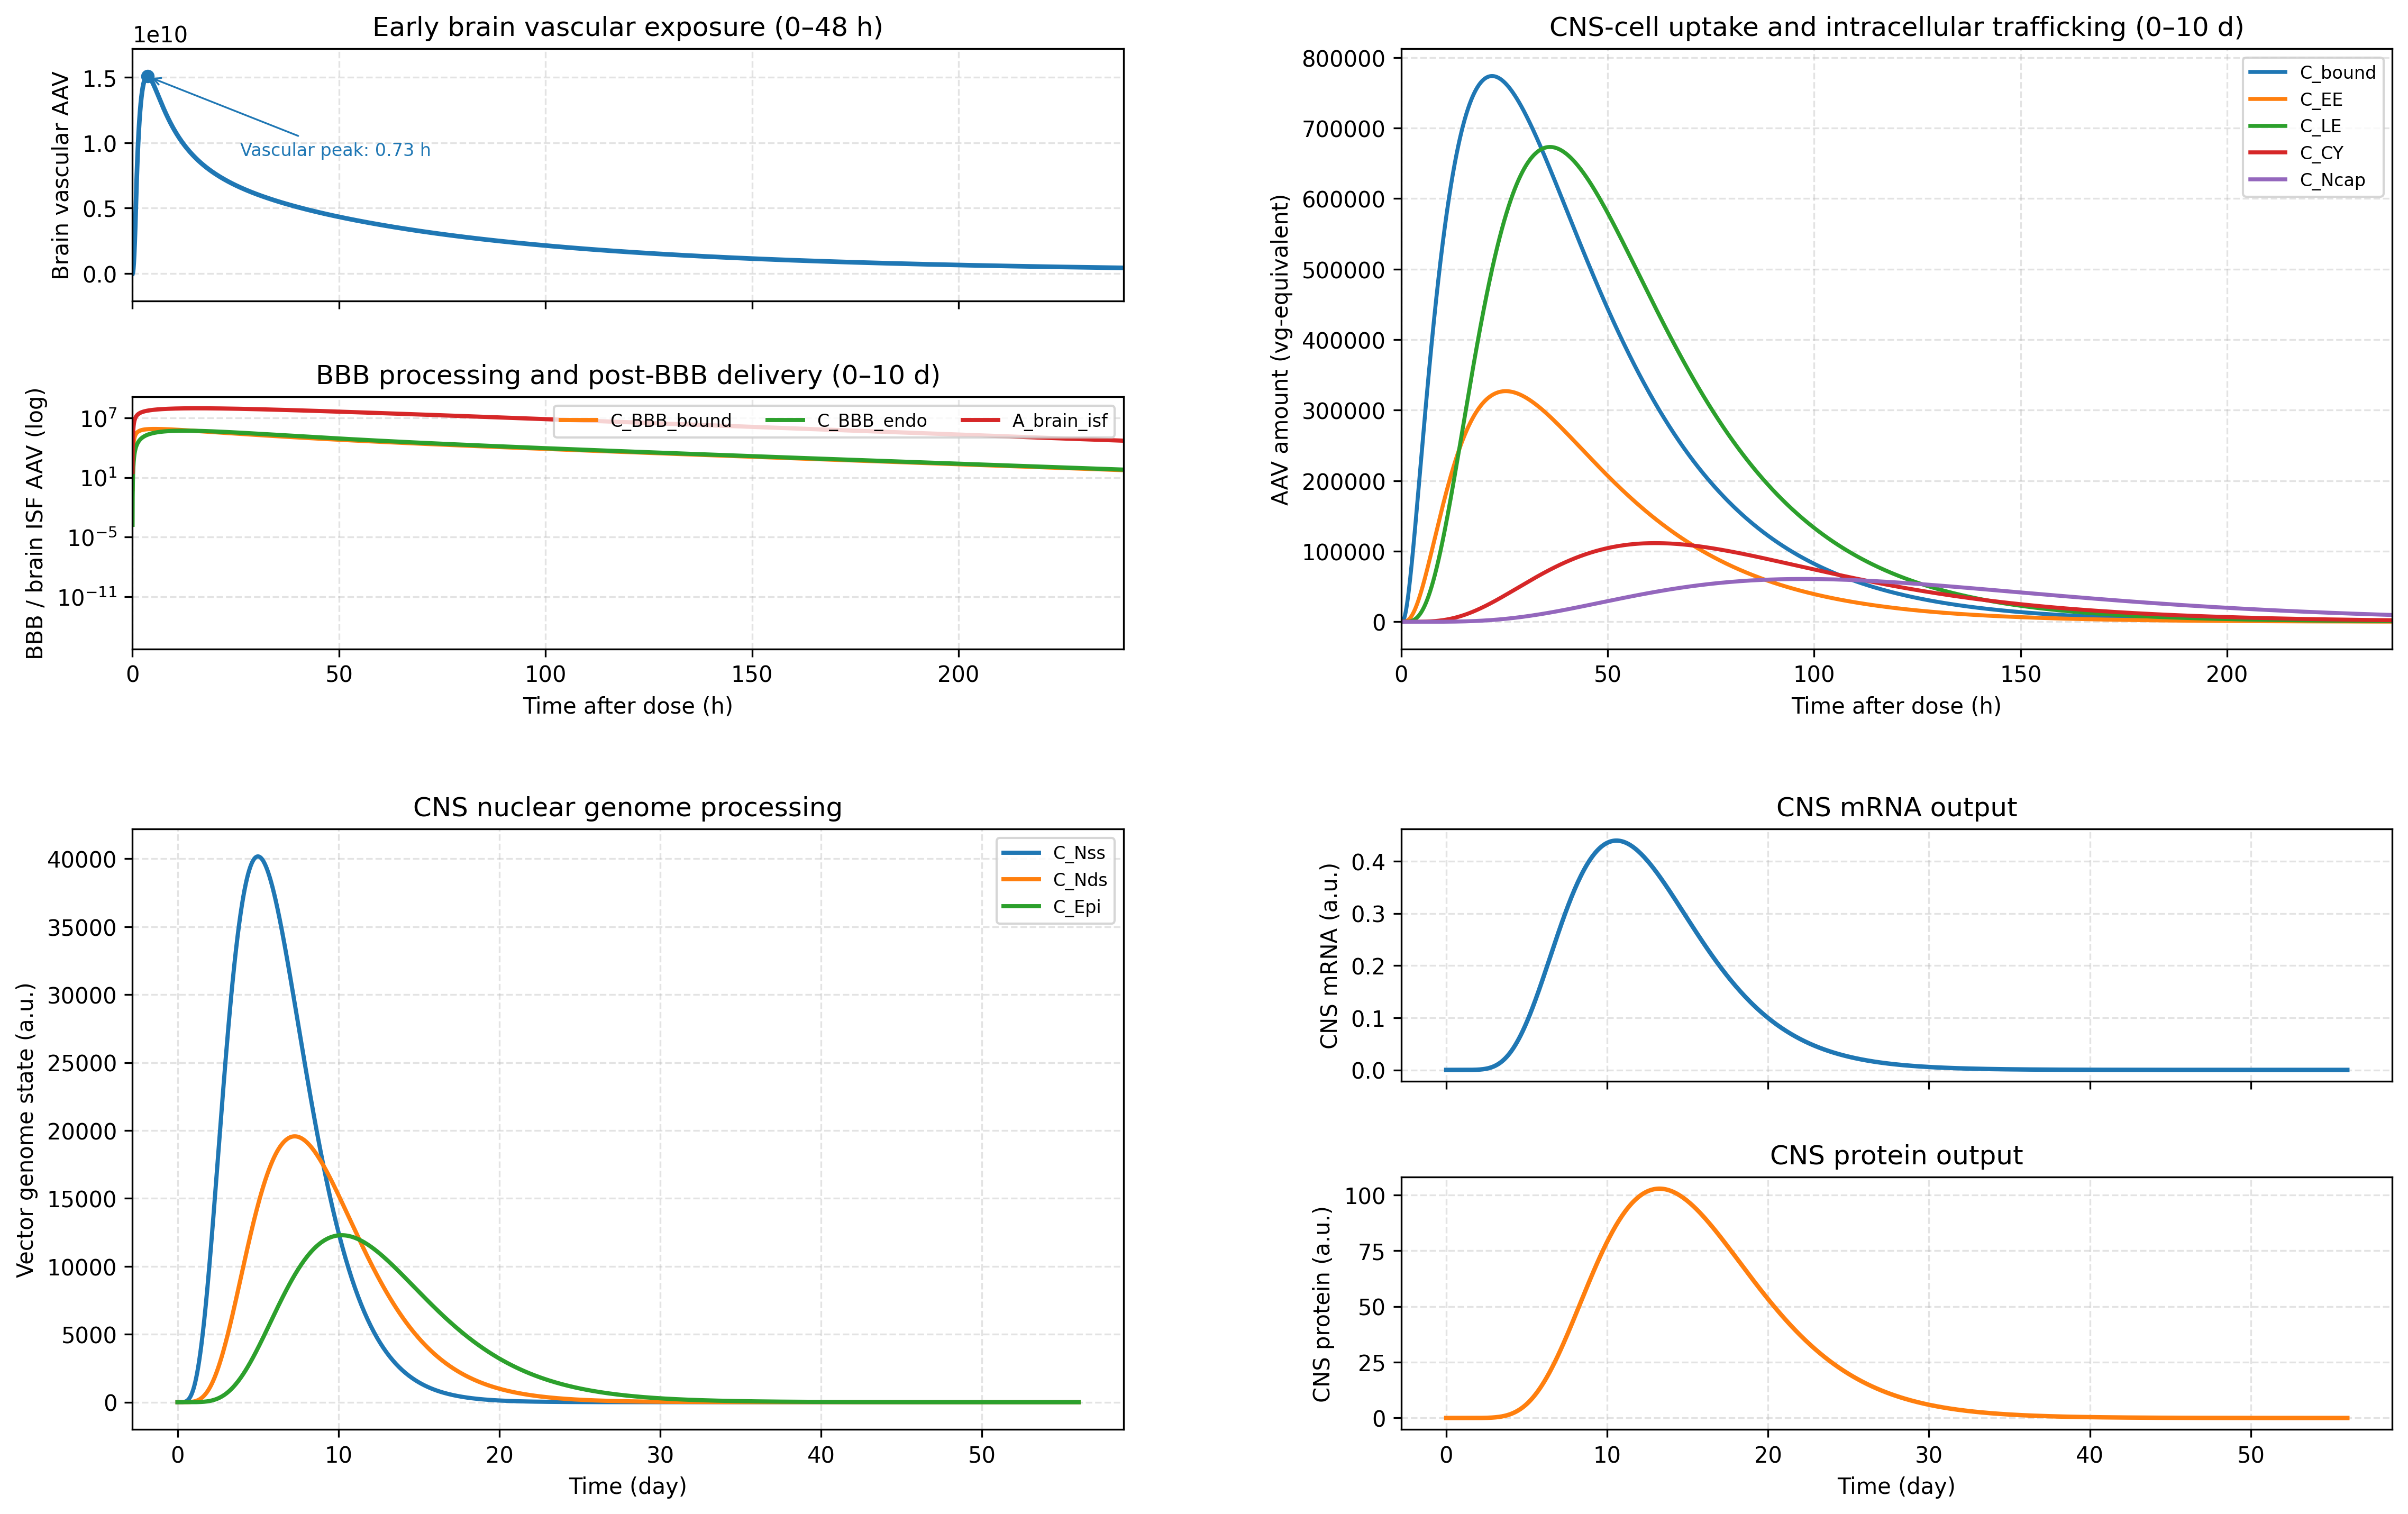
\includegraphics[width=0.98\textwidth]{11_cns_bbb_and_transduction.png}
\caption{CNS 模块输出。脑血管早期峰与 BBB/脑间质小量级状态分开显示；BBB/ISF 使用对数纵轴；mRNA 与蛋白独立成图。}
\end{figure}

基线模型得到脑 ISF amount AUC $5.677\times10^{10}$ vg-equivalent$\cdot$h，约为肝 ISF amount AUC 的 0.92\%；峰值 CNS episome 为 $1.229\times10^4$，峰值蛋白信号为 102.79 a.u.。在演示性的 CNS-tropic 参数组合下，BBB/CNS capsid 增强将峰值 CNS episome 提高到约 $1.336\times10^6$；再叠加 CNS-biased promoter 后，峰值 CNS 蛋白信号达到约 $5.697\times10^3$。这些比较说明屏障跨越、细胞内逃逸和表达调控是可叠加但不等价的设计杠杆。

\subsection{BBB 后三级深度模型}
为了细化求解和更好求解基因表达于各个脑区的不同 CNS 疾病，批量导出器在 $A_{brain,isf}(t)$ 之后继续求解浅表/血管周围层 $S$、皮层实质 $C$ 和深部核团 $D$：
\begin{align}
\dot S &=0.55\,u(t)-(0.18+0.08)S+0.025C,\\
\dot C &=0.18S-(0.025+0.025+0.035)C+0.012D,\\
\dot D &=0.025C-(0.012+0.050)D,
\end{align}
其中 $u(t)=A_{brain,isf}(t)/D_{dose}$。疾病/细胞类型 $j$ 的可接近信号为
\begin{equation}
X_j(t)=a_j\left(w_{S,j}S+w_{C,j}C+w_{D,j}D\right),
\end{equation}
再进入 reduced binding--endosome--cytosol--nucleus--episome ODE。不同 profile 拥有不同深度权重、cell-access factor、目标深度和持久性修正。例如 cortical excitatory 偏浅层和皮层，deep striatal 与 hypothalamic 偏深层，neural progenitor 还加入较低持久性因子。

\assumption{当前三级深度是 reduced-order compartment model，不是脑解剖网格，也没有显式细胞迁移、轴突运输、CSF 循环或区域血流。它用于产生可解释的疾病间差异，并作为未来 3D 模型的降阶原型。}

\section{SINEUP 药效动力学与持久性}

前端的持续时间由 PBPK/胞内 ODE 输出的相对 episome 递送信号驱动一个 0--730 d 的 SINEUP-PD 模型。对同一器官/同一 CNS profile，先将各衣壳的 episome AUC 归一化：
\begin{equation}
E_0=\frac{\AUC_{Epi,capsid}}{\max_c\AUC_{Epi,c}}.
\end{equation}
随后求解
\begin{align}
\dot E &=-k_{loss,E}E,\qquad k_{loss,E}=\frac{\ln2}{t_{1/2,E}},\\
\dot S_{RNA}&=k_{S}\frac{E}{EC_{50,E}+E}-k_{deg,S}S_{RNA},\\
G(S_{RNA})&=G_{max}\frac{S_{RNA}}{EC_{50,S}+S_{RNA}},\\
P_{set}&=\min\left[1,\,0.5(1+G)\right],\\
\dot P&=k_{turn}(P_{set}-P).
\end{align}
基线将单倍剂量不足的蛋白设为 50\%，当预测蛋白达到 65\% 以上时计入有效治疗窗口。网页纵轴使用最后一次高于 65\% 阈值的时间作为 \code{effective\_duration\_days}。当前 SINEUP RNA 半衰期为 0.25 d，目标蛋白半衰期为 2 d，episome 半衰期由器官先验和衣壳 persistence factor 决定。

这套结构的重要意义在于：纵轴同时受初始递送、episome 保持、SINEUP RNA 周转和内源蛋白周转影响，而不是简单把 capsid 半衰期当成疗效持续时间。

\section{数值求解、时间网格与质量守恒}

\subsection{积分策略}
两条 ODE 支路均使用 SciPy \code{solve\_ivp}。鼠模型在 10 min 输注终点处分段积分，避免输入不连续影响峰值；参考成人模型使用刚性 BDF、dense output、相对容差 $2\times10^{-7}$、绝对容差 $10^{-4}$，并将最大步长限制为 24 h。人体时间网格同时解析秒级注射/首过、0--24 h 早期 PK、1--30 d 组织动力学和 31--730 d 持久性。前端仍使用线性 0--72 h 与 1--730 d 两个滑块，通过分段线性插值读取非均匀 ODE 网格；因此显示轴是线性的，但求解在快速变化阶段拥有更密采样。

区域 $T_{max}$ 不只取离散网格中的最大点。导出器利用 dense solution，在采样峰左右区间内对负浓度执行有界标量最小化，从而细化峰值时间。该步骤改善了不同器官达峰时间的比较，但若曲线平台很宽，$T_{max}$ 本身仍可能对噪声和参数不敏感。

\subsection{质量守恒审计}
定义所有仍存在的 AAV 状态与累计损失 sink 之和为 $A_{accounted}$：
\begin{align}
A_{accounted}={}&A_{extracellular}+A_{liver,vector}+A_{kidney,vector}+A_{CNS,vector}\\
&+K_{Urine}+K_{Deg}+C_{Deg}+L_{blood}+L_{vascular}+L_{ISF}+L_{neut}+L_{liver}.
\end{align}
相对误差为
\begin{equation}
\epsilon_{mass}(t)=\frac{A_{accounted}(t)-Dose_{in}(t)}{\max(Dose_{in}(t),10^{-30})}.
\end{equation}
基线鼠模型最终误差为 $-3.418\times10^{-15}$，不同设计场景保持在 $10^{-14}$ 数量级。人体模型则将所有循环池、CSF/depot、24 区域的载体状态和 \code{Loss} 相加，与累计 \code{Dose\_in} 比较；每个途径和衣壳均单独检查。本轮 48 个途径--衣壳组合的最大绝对误差为 $3.493\times10^{-9}$。质量守恒证明 ODE 状态转移在数值上闭合，但\textbf{不能证明参数、人源转化或疗效预测正确}。

\begin{figure}[H]
\centering

\includegraphics[width=0.84\textwidth]{08_mass_balance_audit.png}
\caption{质量守恒审计输出。模型将清除和降解作为显式累计状态，而不是让向量从方程中无去向地消失。}
\end{figure}

\section{衣壳与启动子场景比较}

主模型提供 capsid 与 promoter 两层 preset。capsid 层可改变器官 $PS/K_p$、受体结合、BBB 跨越和内体逃逸；promoter 层只改变 episome 之后的组织表达参数。这样可以避免把“送得更多”和“表达得更多”混成同一个参数。

\begin{table}[H]
\centering
\caption{当前主模型场景结果摘要。数值是模型单位，用于场景内比较。}
\begin{tabularx}{\textwidth}{lrrrr}
\toprule
场景 & 肝峰值 Epi & 肾峰值 Epi & 肝峰值蛋白 & 肾峰值蛋白 \\
\midrule
Baseline & 4,683 & 103,806 & 5,913 & 3,588 \\
Liver detargeted & 2,798 & 100,847 & 5,854 & 3,587 \\
Kidney tropic + kidney promoter & 4,679 & 357,155 & 2,661 & 6,229 \\
Endosomal escape enhanced & 11,562 & 247,864 & 5,962 & 3,592 \\
\bottomrule
\end{tabularx}
\end{table}

例如，增强内体逃逸显著提高了肝和肾 episome，但由于表达 Hill 函数接近饱和，峰值蛋白并未等比例提高。这是机制模型相对于线性评分的优势：它能揭示某个优化是否已被下游瓶颈“截断”。

\begin{figure}[H]
\centering

\includegraphics[width=0.9\textwidth]{09_design_scenario_comparison.png}
\caption{基线、肝脱靶、肾嗜性和内体逃逸增强场景的比较。}
\end{figure}

\section{二维设计空间与疾病数据库}

\subsection{从 ODE 输出到二维坐标}
每个“目标器官/细胞 profile--衣壳”组合形成一个点。横轴是器官特异性：
\begin{equation}
S_{organ}=\log_{10}\left(
\frac{\AUC(C_{target,isf})}
{\operatorname{mean}_{i\ne target}[w_i\AUC(C_{i,isf})]}
\right),
\end{equation}
其中 $w_i$ 是脱靶毒性权重。纵轴是上一节 SINEUP-PD 数值求解得到的有效持续时间。点的详情还显示峰值 post-barrier delivery、目标暴露份额、tmax、证据等级、物种来源、转导模型类型和质量守恒误差。

背景色不是额外修改计算结果，而是把二维空间划分为四个设计语义区：
\begin{itemize}
  \item 高特异性、长持续：优先候选；
  \item 高特异性、短持续：适合需要可逆性或可重复给药的情况；
  \item 低特异性、长持续：需警惕长期脱靶表达；
  \item 低特异性、短持续：通常效用较低。
\end{itemize}

\subsection{衣壳先验与证据标签}
当前数据库包含 AAV2、AAV5、AAV8、AAV9、AAVrh.10、PHP.eB、CAP-B10 和 AAV-LK03。先验通过缩放器官 $PS_i$、$K_{p,i}$ 和 BBB transcytosis 映射到 PBPK，而不是直接手填最终二维坐标。不同来源跨越 mouse、NHP、human-hepatocyte prior 和临床/局部眼科证据，因此前端明确显示 strong、medium、exploratory，并保留 source 链接。PHP.eB 等衣壳的物种依赖尤其需要显著提示，不能将特定小鼠受体背景中的 CNS 嗜性直接外推到人。

\subsection{疾病--基因层级库}
疾病库采用“疾病列表--展开基因”的层级结构，当前约含 27 个疾病组、44 条疾病--基因记录和 42 个唯一基因。Wolf--Hirschhorn syndrome 不再是单一记录，而是包含 NSD2、LETM1、MSX1、FGFR3 和 CPLX1；同时加入 CHD8、SCN1A/Dravet、SHANK3/Phelan--McDermid、EHMT1/Kleefstra、RAI1/Smith--Magenis、NSD1/Sotos、SATB2、MEF2C、FOXP1、TCF4、SYNGAP1、DYRK1A、NRXN1、PAFAH1B1、ANKRD11 等单倍剂量不足或缺失相关疾病。每条记录包含 locus、目标器官、目标细胞、机制、残余等位基因要求、注意事项和 ClinGen/综述证据入口。

CNS 疾病会进一步映射到 cortical excitatory、cortical inhibitory、cortical projection、synaptic neuron、deep striatal、hypothalamic、broad neuronal 或 neural progenitor profile。于是同一衣壳在不同疾病中会因目标深度和细胞可接近性而得到不同的特异性及持续性，不再是一套数据复用。

\subsection{GTEx 与 Human Protein Atlas 表达证据}
脚本首先从疾病库抽取唯一基因符号，经 GTEx reference API 转换为 GENCODE v39 ID，再读取 GTEx v10 的组织中位 TPM。脑、心、肝、肾、骨骼肌和肺的细分组织按模型器官聚合并取中位数。GTEx 提供健康成人 bulk-tissue RNA 先验\cite{gtex2020}；Human Protein Atlas（HPA）补充 RNA tissue specificity、RNA distribution 与 protein tissue specificity\cite{hpa2015}。组织特异性指数为
\begin{equation}
\tau=\frac{\sum_{i=1}^{n}(1-x_i/x_{max})}{n-1},
\end{equation}
其中 $\tau\to1$ 表示表达集中在少数组织，$\tau\to0$ 表示广泛表达。GTEx TPM 进入组合筛选的弱修正项，HPA 与 $\tau$ 当前主要用于证据展示和交叉检查。它们不能证明患者残余等位基因仍有足量转录本，也不能替代细胞类型、发育阶段或患者来源样本。

\subsection{单方案与双方案组合筛选}
组合筛选使用人体模型汇总的 48 个候选，即 6 条途径 $\times$ 8 种衣壳。对目标器官，先定义
\begin{equation}
R=\log_{10}(\AUC_{ISF}+1)+0.35\log_{10}(P_{peak}+1),
\end{equation}
并在该器官的全部候选间做 min--max 归一化得到递送强度 $D$。目标器官 AUC 份额转为
\begin{equation}
S=\min\left(1,\frac{Share_{target}}{45\%}\right).
\end{equation}
基因 $g$ 的健康组织表达修正为
\begin{equation}
E_g=\operatorname{clip}\left[
\frac{\log(1+TPM_{target,g})}{\log(1+TPM_{max,g})},0.15,1
\right],
\end{equation}
最终单基因覆盖分数为
\begin{equation}
G_g=(0.72D+0.28S)(0.65+0.35E_g).
\end{equation}
单方案取同一疾病全部可建模基因的 $G_g$ 均值，再扣除给药途径负担。双方案对每个基因取 $\max(G_{A,g},G_{B,g})$，避免把两个独立全剂量求解结果错误相加，再扣除两次给药和衣壳免疫惩罚。只有双方案比最佳单方案至少高 0.10 才显示。当前 $0.35$、$0.72/0.28$、45\%、途径负担和免疫惩罚都是显式工程规则，不是拟合出的治疗成功概率；同一疾病内的核心基因与候选修饰基因暂时也采用相同权重。

\subsection{两条计算支路的边界}
当前二维“特异性--持久性”散点来自鼠尺度 \code{ode1.0.py}、CNS 三级深度模型与 SINEUP-PD；人体分区热图来自 301 状态参考成人模型；组合筛选则使用人体模型按父器官汇总的 route--capsid 指标。因此三块界面已经共享方程族和衣壳先验，但尚未完全共享同一套人体细胞参数。下一版应直接用人体 24 区域轨迹生成二维点和 SINEUP-PD，并在同一个 ODE 中联合求解剂量拆分、竞争和免疫相互作用。

\subsection{前端实现与数据来源证明}
前端采用中英文切换、独立可滚动疾病库、可展开疾病组、全部衣壳切换、模型/代理标签和证据卡。导出器当前生成 48 个器官级设计点、64 个 CNS profile 点、64 个鼠器官热图点和 1152 个途径--衣壳--人体区域点，共 1328 个输出。网页读取版本化 JSON，不在浏览器中运行 SciPy；人体轨迹按时间插值后映射到分层 SVG。颜色对 share/$T_{max}$ 使用线性尺度，对浓度、AUC、episome 与 protein 使用跨同途径全部衣壳/区域的对数尺度，因此颜色表达相对排序，右侧数值才是原始模型量。模型生成时间固定为 UTC 字符串，避免本地时区导致 React hydration mismatch。

\section{Spatial PK 与流体力学路线}

\subsection{已完成的一维演示}
当前一维模型在归一化血管/组织轴 $x$ 上求解对流--扩散--受体摄取：
\begin{equation}
\frac{\partial C}{\partial t}+u\frac{\partial C}{\partial x}
=D\frac{\partial^2C}{\partial x^2}-J_{uptake}(C,B),
\end{equation}
并在每个网格点计算
\begin{align}
\dot B&=k_{on}C(B_{max}-B)-k_{off}B-k_{int}B,\\
\dot I&=k_{int}B-k_{escape}I-k_{lys}I,\\
\dot E&=k_{escape}I-k_{loss,E}E.
\end{align}
入口边界 $C(0,t)$ 来自 0D PBPK 的血液浓度曲线。演示比较 baseline IV-like、capsid wall-access enhanced 和 slow-flow local trapping，说明即使总给药相同，流速、停留时间和壁面摄取也会改变最终 episome 的空间均匀度。

\begin{figure}[H]
\centering

\includegraphics[width=0.88\textwidth]{10_spatial_pk_1d_demo.png}
\caption{一维 spatial PK 演示：PBPK 作为入口边界，局部流动和壁面摄取共同塑造表达性 episome 的空间分布。}
\end{figure}

\subsection{未来 3D CNS 模型}
下一阶段可建立从血管到脑实质的 3D advection--diffusion--reaction 模型：
\begin{align}
\nabla\cdot\bm u&=0,\\
\rho\left(\frac{\partial\bm u}{\partial t}+\bm u\cdot\nabla\bm u\right)&=-\nabla p+\mu\nabla^2\bm u,\\
\frac{\partial C}{\partial t}+\nabla\cdot(\bm uC)&=\nabla\cdot(D\nabla C)-R_{uptake}(C,\bm x).
\end{align}
推荐分四步实施：
\begin{enumerate}
  \item 用理想化毛细血管--周血管--实质圆柱几何完成 2D axisymmetric 原型；
  \item 将 BBB 通量设为 Robin 边界，参数由当前 ODE 的 $k_{BBB}$ 和受体容量转换；
  \item 加入脑区分层的扩散系数、细胞密度、受体密度和外排/降解；
  \item 使用成像或组织切片校准空间参数，再导出降阶参数回填网页的 CNS profile。
\end{enumerate}
若有 MRI/血管图谱，可进一步构建个体化几何；若没有，先用理想化微血管单元比直接上全脑网格更容易验证。对 CSF 或局部脑内给药，还需加入 CSF bulk flow、pulsatility 和 perivascular transport。PET 研究表明，即使向 CSF 给药，也可能有显著系统外流和外周器官暴露，因此未来模型必须同时保留 CNS 与全身收支\cite{csfpet2023}。

\section{Measurement 与湿实验闭环}

测量设计首先区分 measurand：完整/标记 capsid 用于早期 capsid PK，qPCR/ddPCR vector genome 用于组织载量，核内环状或双链状态用于 episome，RT-qPCR 用于 SINEUP RNA，定量蛋白或功能 assay 用于药效。它们不能共用一个“半衰期”。建议至少报告单位、样本基质、回收率、标准曲线、定量下限、生物学与技术重复、原始值及不确定性。

\begin{table}[H]
\centering
\caption{模型参数、可测量数据与实验反馈关系。}
\begin{tabularx}{\textwidth}{p{0.22\textwidth}p{0.30\textwidth}X}
\toprule
模型环节 & 推荐实验 & 可校准参数/判别问题 \\
\midrule
血液与器官分布 & 血浆及肝/脾/肾/心/肌/肺/脑 qPCR 或 ddPCR 时间序列 & $Q_i,PS_i,K_{p,i},k_{clear}$；区分早期分布与后期残留 \\
完整 capsid 命运 & capsid ELISA/免疫染色、放射或荧光标记成像 & 表观 capsid PK；避免仅用 vg 信号解释完整病毒 \\
细胞类型摄取 & 组织切片与 hepatocyte、Kupffer、PT、endothelium、neuron/glia marker 共定位 & $B_{max},k_{on},k_{int}$ 及细胞类型份额 \\
胞内运输 & 亚细胞分级、内体/溶酶体/核共定位 & $k_{escape},k_{lys},k_{nuc},k_{uncoat}$ \\
episome & 核内 vector genome、双链/环状 episome 测定 & $k_{ds},k_{epi},k_{loss,Epi}$ \\
SINEUP RNA & RT-qPCR、RNA half-life、构建特异表达 & $k_{S},k_{deg,S}$，不同 SINEUP 元件比较 \\
蛋白恢复 & western blot、ELISA、功能 readout & 翻译增益、蛋白周转、65\% 阈值的生物学合理性 \\
空间分布 & 全器官成像、分区取样、空间转录/蛋白检测 & $D,u,R_{uptake}$ 与 CNS 深度权重 \\
免疫 & NAb、补体、细胞因子及重复给药实验 & $k_{neut}$、免疫清除和重复给药限制 \\
\bottomrule
\end{tabularx}
\end{table}

推荐最小闭环是：先选择 2--3 个衣壳、1 个报告系统和肝/肾/脑三个组织，在 0.5 h、2 h、8 h、24 h、72 h、7 d 和 28 d 取样。早期测 vector/capsid，后期测 episome、RNA 和蛋白。用早期数据拟合 PBPK 与摄取，用后期数据拟合表达和持久性，再重新生成二维点图。这样网页中的候选排序会随实验数据更新，而不是停留在固定文献先验。

\section{AAV 安全性研究与当前模型边界}

安全性不能由“模拟剂量低于某上市产品剂量”推出。风险还受总 capsid、full/empty ratio、衣壳、启动子、payload、杂质、途径、年龄、疾病和既往免疫影响。本人体演示剂量为 $4.0\times10^{13}$ vg/kg；ZOLGENSMA 标签中的 $1.1\times10^{14}$ vg/kg 只作为 AAV9 静脉给药的临床背景，不能当成通用安全阈值\cite{zolgensma2026}。

\begin{table}[H]
\centering
\caption{当前优先关注的 AAV 风险及其测量端点。}
\begin{tabularx}{\textwidth}{p{0.19\textwidth}p{0.32\textwidth}X}
\toprule
风险域 & 已知背景 & 本项目应测量/建模 \\
\midrule
肝毒性 & 系统 AAV 常见风险，可表现为转氨酶升高、严重肝损伤或衰竭 & 肝 capsid/transgene AUC、ALT/AST、胆红素、白蛋白、PT/INR、抗 capsid T 细胞 \\
血小板减少/TMA & AAV9 后报告微血管血栓、溶血、血小板减少与急性肾损伤 & 血小板、血红蛋白、肌酐、尿检、LDH/结合珠蛋白及补体 \\
心脏信号 & onasemnogene abeparvovec 需关注 troponin 升高 & 心脏暴露、troponin 与必要的心脏评估 \\
CNS/DRG & CSF/局部 AAV 项目出现 DRG 病理或局部 MRI 改变 & 神经/感觉终点、MRI、CSF marker 及相关动物 DRG 病理 \\
免疫与 CMC & NAb 可降低首次疗效；空壳、宿主残留和内毒素可改变风险 & NAb、T 细胞、细胞因子、补体、full:empty、效价、纯度和器械相容性 \\
\bottomrule
\end{tabularx}
\end{table}

FDA 的临床开发材料把 IV AAV 与肝毒性/TMA、IT 或脑实质给药与 DRG/局部神经毒性联系起来\cite{fdaaav2023}。本项目新增的 safety screen 只将每个 route--capsid 的器官 AUC 与同模型 IV-AAV9 比较，用来决定优先增加哪些 assay；它没有 AUC 到 ALT、TMA、troponin 或神经损伤的校准函数，因此不会输出“安全/不安全”。下一步应在同一产品或同一研究系列中拟合非线性 exposure--response，并保留不确定区间。

\section{Attribution 与可复用 Contribution}

Git 历史显示当前仓库实现由朱子轩完成，包括 PBPK/ODE、人体区域模型、批量导出、疾病/基因界面、参数证据整理与可视化。生物学参数、数据、软件和解剖图均来自外部工作，不属于团队原创实验数据；Reactome 解剖 SVG 按 CC BY 4.0 记录原作者和修改方式。Codex/OpenAI 工具参与代码与文档辅助，所有科学判断和最终提交仍需学生作者核验。指导、湿实验、RNA binder 模型、wiki 美术和机构支持的人名及具体贡献必须由全队在官方 Attributions Form 中逐项确认，本文不代为虚构。

本项目为未来队伍提供两项主要贡献：其一，\code{export\_parameter\_registry.py} 将实际进入方程的参数导出为 CSV、JSON 和 LaTeX，并为每项记录 unit、species、source、direct/fitted/derived/scaled/assumed、confidence 和 calibration priority；其二，提供从 PBPK/胞内 ODE 到版本化 JSON/CSV，再到疾病库、二维设计空间和分层人体 SVG 的复现流程。贡献的价值在于其他队伍可以替换自己的测量数据，而无需重新搭建整条计算链。

\section{当前结果应该如何解释}

\subsection{可以支持的结论}
\begin{itemize}
  \item 模型在结构上连接了系统暴露、屏障跨越、细胞摄取、胞内运输和表达输出；
  \item 参考成人模型能够比较不同给药入口、心肺首过、CSF 回流和 24 个区域的相对时序；
  \item 普通 AAV9-like 参数下，脑间质暴露显著低于肝脏，BBB 是明确瓶颈；
  \item 肾脏不能只用“滤过”解释，基底外侧摄取和胞内分流会显著改变转导；
  \item 内体逃逸增强可显著增加 episome，但蛋白输出可能因下游饱和而增幅有限；
  \item 衣壳、启动子和局部流动作用于不同层级，应分别优化；
  \item 二维图适合做候选筛选和实验优先级排序。
\end{itemize}

\subsection{目前不能支持的结论}
\begin{itemize}
  \item 不能把当前 vg-equivalent 或 a.u. 直接换算为人体治疗剂量；
  \item 不能将放射标记 capsid 半衰期等同于感染性 capsid、vector genome 或表达持续时间；
  \item 不能把小鼠衣壳 tropism 直接外推到 NHP 或人；
  \item 不能仅凭器官 AUC 预测 CNS 细胞类型疗效；
  \item 不能将 Eye、Heart、Muscle 的 reduced surrogate 与肝/肾/CNS 原生胞内 ODE 视为同等证据；
  \item 不能把 GTEx 成人 bulk TPM 当作目标神经元表达或患者残余转录本证据；
  \item 不能把组合覆盖分数解释为治疗成功率，也不能据此直接确定联合剂量；
  \item 不能把 70 kg 标签理解为已经完成临床标定；有效流量缩放、CSF/局部 depot 和衣壳人源转化仍是待拟合先验；
  \item 不能用质量守恒误差很小来证明生物学参数正确。
\end{itemize}

\section{代码组织、复现与跨电脑展示}

\subsection{核心文件}
\small
\begin{longtable}{>{\raggedright\arraybackslash}p{0.40\textwidth}>{\raggedright\arraybackslash}p{0.50\textwidth}}
\toprule
文件/目录 & 作用 \\
\midrule
\endfirsthead
\toprule
文件/目录 & 作用 \\
\midrule
\endhead
\path{model/ode1.0.py} & 全身 PBPK、肝/肾/CNS 胞内 ODE、场景模拟、质量守恒和绘图 \\
\path{model/human_spatial_pbpk.py} & 70 kg、24 区域、301 状态、多给药途径人体参考模型 \\
\path{model/export_delivery_design_space.py} & 批量运行两条支路，计算 CNS 深度、SINEUP-PD、人体汇总并输出 JSON/CSV \\
\path{model/export_parameter_registry.py} & 输出完整参数证据注册表 \\
\path{results/mouse_pbpk/} & 当前模型图片及指标 CSV \\
\path{sineup-delivery-atlas/app/} & 疾病库、二维设计空间、组合筛选和人体分层 SVG 前端 \\
\path{sineup-delivery-atlas/public/data/} & ODE 与 GTEx/HPA 的版本化 JSON/CSV 快照 \\
\path{docs/} & 建模报告、汇报材料和本 LaTeX 源文件 \\
\bottomrule
\end{longtable}
\normalsize

\subsection{推荐迁移流程}
当前仓库把现行模型放在 \path{model/}，报告放在 \path{docs/latex/}，旧脚本保留在 \path{archive/legacy/}。前端以普通目录纳入同一仓库，因此一个 commit 可以同时恢复模型、数据和网页。

仅用于展示时，预生成的三个数据文件已经包含模型轨迹和表达证据，另一台电脑只需 Git 和 Node.js $\ge22.13$：
\begin{lstlisting}[language=bash]
git clone https://github.com/zzx060827/iGEM_ODE.git
cd iGEM_ODE/sineup-delivery-atlas
npm ci
npm run dev
\end{lstlisting}
浏览器访问终端显示的本地地址即可。正式演示建议提前执行 \code{npm run build}，并保留无网络可用的数据快照。

若需要在新电脑重新求解 ODE，再创建 Python 环境并将输出直接写入前端数据目录：
\begin{lstlisting}[language=bash]
conda create -n transformer python=3.11 \
  numpy scipy matplotlib -y
conda activate transformer

python model/export_parameter_registry.py
python model/export_delivery_design_space.py \
  --model model/ode1.0.py \
  --output sineup-delivery-atlas/public/data/model-results.json

cd sineup-delivery-atlas
npm ci
npm run dev
\end{lstlisting}
导出命令会同步产生 \path{model-results.json}、\path{model-results.csv} 和 \path{human-spatial-results.json}；GTEx/HPA 缓存可用 \code{npm run data:expression} 单独刷新。展示机若只读取已提交 JSON，不需要安装 Conda。

\subsection{可复现性清单}
\begin{itemize}
  \item 固定 Python/Node 版本并补充 \code{environment.yml} 或 \code{requirements.txt}；
  \item 在数据 JSON 中保留生成时间、模型 commit、参数版本和参考物种；
  \item 将文献先验、拟合参数与演示参数放入分开的表；
  \item 自动检查 ODE 成功状态、非负性、质量守恒和输出文件；
  \item 前端只消费已版本化模型输出，不在客户端使用随机数或本地时区生成首屏文本；
  \item 为答辩准备无网络本地版本和已生成 PDF/PNG 结果。
\end{itemize}

\section{下一阶段路线图}

\begin{enumerate}
  \item \textbf{参数分层：}将 physiology、capsid、cell-fate、immune、PD 和 numerical settings 拆成独立配置，并为每个参数增加 unit、species、source、confidence。
  \item \textbf{校准接口：}读取实验 CSV，用最小二乘或 Bayesian 方法估计 $PS,K_p,k_{res},k_{escape},k_{epi}$，输出置信区间和可辨识性。
  \item \textbf{统一两条支路：}用人体 24 区域轨迹直接生成二维设计点和 SINEUP-PD，并把鼠肾近端小管专门机制嵌入人体肾皮质。
  \item \textbf{数据层：}将当前静态 TypeScript/JSON 迁移为可查询的 disease--gene--cell--capsid 数据库，保留 PMID/DOI、实验物种、给药途径、剂量、时间点和 assay。
  \item \textbf{不确定性：}进行 Latin hypercube/Monte Carlo 和 Sobol sensitivity，二维点显示置信椭圆而非单点。
  \item \textbf{免疫模块：}将 NAb、补体、Kupffer/splenic uptake 和重复给药影响加入显式状态。
  \item \textbf{CNS 空间模型：}从理想化 2D 微血管单元开始，再升级至区域化 3D 几何；用实验空间分布校准。
  \item \textbf{多目标优化：}在目标表达、脱靶 AUC、剂量、免疫风险和空间均匀性之间计算 Pareto front；为核心致病基因与候选修饰基因设置不同证据权重。
  \item \textbf{湿实验闭环：}每轮实验更新参数后自动重跑、导出数据并刷新前端，形成真正的 design--build--test--learn 循环。
\end{enumerate}

\section{参数证据说明}

完整逐参数表位于配套技术附录；机器可读版本为 \path{model/data/model_parameter_registry.csv}。最需要优先校准的是有效流量缩放、器官 $PS/K_p$、血管/ISF 损失拆分、BBB/CSF access、肾双入口、内体逃逸、episome persistence 和 SINEUP gain；人体血容量、CSF 容积/生成量和直接转录的 AAV9 早期 PET 半衰期具有相对更强的外部依据。

\section{汇报用结论}

本项目已经从“让 AAV 曲线出现峰值和衰减”的单器官演示，发展为 64 状态鼠机制模型、301 状态参考成人模型、表达证据库和 React 决策界面组成的多尺度平台。模型最重要的升级不是增加更多曲线，而是建立从疾病靶点、给药入口和系统分布到最终蛋白恢复的因果链：PBPK 决定器官入口，受体和屏障决定细胞可达性，胞内运输决定 episome，SINEUP-PD 决定蛋白恢复及持续时间，spatial PK 决定同一器官内部是否均匀到达。二维前端与人体热图把这条链转化为可检查来源、假设和证据强度的交互工具。

当前工作适合用于 iGEM 展示、机制假设比较和湿实验优先级设计。最严谨的表述是：疾病库定义“需要送到哪里”，GTEx/HPA 判断“健康组织中是否存在目标转录本先验”，PBPK 计算“如何到达”，胞内 ODE 计算“到达后有多少形成表达状态”，SINEUP-PD 计算“可能恢复多少和维持多久”，评分层再比较单方案与组合方案。下一步的科学重点是统一人体计算支路，并用早期分布、细胞共定位、episome、RNA 和蛋白数据完成校准与不确定性分析。

\clearpage
\begin{thebibliography}{99}

\bibitem{pbpk2024}
Liu S, Chowdhury EA, Xu V, et al. Whole-Body Disposition and Physiologically Based Pharmacokinetic Modeling of Adeno-Associated Viruses and the Transgene Product. \textit{J Pharm Sci}. 2024;113(1):141--157. \href{https://doi.org/10.1016/j.xphs.2023.10.005}{doi:10.1016/j.xphs.2023.10.005}.

\bibitem{ballon2020}
Ballon DJ, Rosenberg JB, Fung EK, et al. Quantitative Whole-Body Imaging of I-124-Labeled Adeno-Associated Viral Vector Biodistribution in Nonhuman Primates. \textit{Hum Gene Ther}. 2020;31(23--24):1237--1259. \href{https://doi.org/10.1089/hum.2020.116}{doi:10.1089/hum.2020.116}.

\bibitem{pillay2016}
Pillay S, Meyer NL, Puschnik AS, et al. An essential receptor for adeno-associated virus infection. \textit{Nature}. 2016;530:108--112. \href{https://doi.org/10.1038/nature16465}{doi:10.1038/nature16465}.

\bibitem{trafficking2012}
Nonnenmacher M, Weber T. Intracellular transport of recombinant adeno-associated virus vectors. \textit{Gene Ther}. 2012;19:649--658. \href{https://doi.org/10.1038/gt.2012.6}{doi:10.1038/gt.2012.6}.

\bibitem{trafficking2021}
Riyad JM, Weber T. Intracellular trafficking of adeno-associated virus (AAV) vectors: challenges and future directions. \textit{Gene Ther}. 2021. \href{https://doi.org/10.1038/s41434-021-00243-z}{doi:10.1038/s41434-021-00243-z}.

\bibitem{engineering2020}
Li C, Samulski RJ. Engineering adeno-associated virus vectors for gene therapy. \textit{Nat Rev Genet}. 2020;21:255--272. \href{https://doi.org/10.1038/s41576-019-0205-4}{doi:10.1038/s41576-019-0205-4}.

\bibitem{immunity2020}
Vandamme C, Adjali O, Mingozzi F. Unraveling the complex story of immune responses to AAV vectors trial after trial. \textit{Hum Gene Ther}. 2017;28:1061--1074. \href{https://doi.org/10.1089/hum.2017.150}{doi:10.1089/hum.2017.150}.

\bibitem{bioanalytical2023}
PK/PD and Bioanalytical Considerations of AAV-Based Gene Therapies: an IQ Consortium Industry Position Paper. 2023. \href{https://pubmed.ncbi.nlm.nih.gov/37523051/}{PubMed 37523051}.

\bibitem{megalin2002}
Christensen EI, Birn H. Megalin and cubilin: multifunctional endocytic receptors. \textit{Nat Rev Mol Cell Biol}. 2002;3:256--266. \href{https://doi.org/10.1038/nrm778}{doi:10.1038/nrm778}.

\bibitem{sineup2015}
Zucchelli S, Fasolo F, Russo R, et al. SINEUPs: a new class of natural and synthetic antisense long non-coding RNAs that activate translation. \textit{RNA Biol}. 2015. \href{https://pubmed.ncbi.nlm.nih.gov/26259533/}{PubMed 26259533}.

\bibitem{csfpet2023}
Positron Emission Tomography Quantitative Assessment of Off-Target Whole-Body Biodistribution of I-124-Labeled Adeno-Associated Virus Capsids Administered to Cerebral Spinal Fluid. 2023. \href{https://pubmed.ncbi.nlm.nih.gov/37624734/}{PubMed 37624734}.

\bibitem{pbpkprinciples2013}
Jones H, Rowland-Yeo K. Basic concepts in physiologically based pharmacokinetic modeling in drug discovery and development. \textit{CPT Pharmacometrics Syst Pharmacol}. 2013;2:e63. \href{https://doi.org/10.1038/psp.2013.41}{doi:10.1038/psp.2013.41}.

\bibitem{capsidml2021}
Bryant DH, Bashir A, Sinai S, et al. Deep diversification of an AAV capsid protein by machine learning. \textit{Nat Biotechnol}. 2021;39:691--696. \href{https://doi.org/10.1038/s41587-020-00793-4}{doi:10.1038/s41587-020-00793-4}.

\bibitem{gtex2020}
The GTEx Consortium. The GTEx Consortium atlas of genetic regulatory effects across human tissues. \textit{Science}. 2020;369(6509):1318--1330. \href{https://doi.org/10.1126/science.aaz1776}{doi:10.1126/science.aaz1776}.

\bibitem{hpa2015}
Uhl\'{e}n M, Fagerberg L, Hallstr\"{o}m BM, et al. Tissue-based map of the human proteome. \textit{Science}. 2015;347(6220):1260419. \href{https://doi.org/10.1126/science.1260419}{doi:10.1126/science.1260419}.

\bibitem{gray2013}
Gray SJ, Nagabhushan Kalburgi S, McCown TJ, Jude Samulski R. Global CNS gene delivery and evasion of anti-AAV-neutralizing antibodies by intrathecal AAV administration in non-human primates. \textit{Gene Ther}. 2013;20:450--459. \href{https://pmc.ncbi.nlm.nih.gov/articles/PMC3618620/}{PMCID: PMC3618620}.

\bibitem{zolgensma2026}
US National Library of Medicine. ZOLGENSMA (onasemnogene abeparvovec-xioi) Prescribing Information. DailyMed, accessed August 2026. \href{https://dailymed.nlm.nih.gov/dailymed/lookup.cfm?setid=68cd4f06-70e1-40d8-bedb-609ec0afa471}{DailyMed label}.

\bibitem{fdaaav2023}
US Food and Drug Administration. Clinical Development of Gene Therapy Products: examples of toxicities associated with AAV-based products. 2023. \href{https://www.fda.gov/media/167536/download}{FDA presentation}.

\end{thebibliography}

\end{document}
